% arara: pdflatex: { shell: true, draft: true }
% arara: makeglossaries
% arara: biber
% arara: pdflatex: { shell: true, synctex: true }
% arara: pdflatex: { shell: true, synctex: true }

\documentclass[12pt,DIV14,BCOR10mm,a4paper,twoside,parskip=half-,headsepline,headinclude,english,ngerman,bibliography=totocnumbered]{scrreprt}

\usepackage{hshhelper_base}

%%%%%%%%%%%%%%%%%%%%%%%%%%%%%%%%%%%%%%%%%%%%%%%%%%%%%%%%%%%%%%%%%%%%%%%%%%
\begin{document}    % hier gehts los
  \thispagestyle{empty} % Titelseite

\includegraphics[width=0.2\textwidth]{Wortmarke_WI_schwarz}

   {  ~ \sffamily
  \vfill
  {\Huge\bfseries Test-Driven Development in Entwicklungsprozess \enquote{Scrum}}
  \bigskip

  {\Large
  Dennis Grabowski, B.Sc. \\[2ex]
  Projekt- \& Qualitätsmanagement \\
  Wintersemester 18/19
 \\[5ex]
   \today }
}
 \vfill

  ~ \hfill
  
\includegraphics[height=0.3\paperheight]{H_WI_Pantone1665}

\vspace*{-3cm}

\tableofcontents  % Inhaltsverzeichnis

\chapter{Einleitung}

Agile Softwareentwicklungsprozesse sind bereits länger im \enquote{Trend}.
Die drei bekanntesten sind allerdings \enquote{Scrum}, \enquote{Kanban} und \enquote{eXtreme Programming (XP)}.
Laut einem \enquote{Google Trend}-Vergleich scheint sich Scrum allerdings gegenüber seinen \enquote{Konkurrenten} gut gehalten zu haben. \footnote{Siehe \url{https://trends.google.com/trends/explore?date=all\&geo=US\&q=\%2Fm\%2F02zhbn,\%2Fm\%2F0ck\_p8,\%2Fm\%2F02t2n,\%2Fm\%2F0dgq419}}

Alle drei Prozesse basieren auf dem sogenannten \enquote{Agile Manifesto} \autocite{AgileManifesto}. \\
Das Manifesto macht keine genauen Angaben dazu, wie ein agiler Softwareentwicklungsprozess struktuiert werden sollte.
Daher ähneln sich diese drei Prozesse auch nur in den Werten, die sie von dem Agile Manifesto vermittelt bekommen haben.
Oftmals konzentrieren sich diese Prozesse daher auf eine lockere, freie Anforderungsanalyse, um die sogenannte \enquote{Agilität} bieten zu können, oder geben vor, wie die Implementierungsphase aufgebaut ist, da kleinere, aber dafür funktionierende Softwareartefakte (Minimum Viable Product) bevorzugt werden.
Die Testphase wird vom Agile Manifesto nicht aufgegriffen, und fällt daher oftmals in Vergessenheit.  \\
Kanban beschreibt keine Richtlinien bezüglich Tests oder einer Testphase.
Dieser Entwicklungsprozess konzentriert sich auf das visuelle Management durch ein sogenanntes \enquote{Kanban-Board}, welches dabei helfen soll, den Status verschiedener Arbeitspakete zu vermitteln und somit Entscheidungen über diese einfacher treffen zu können.
Aufgrund des Kanban-Boards wird dieser Prozess oftmals mit einem anderen agilen Softwareentwicklungsprozess verknüpft.  \\
Dem gegenüber stehenden ist der Entwicklungsprozess Scrum, der oftmals als ein \enquote{Framework} für Entwicklungsprozesse betrachtet wird.
Scrum definiert einen Entwicklungszyklus, gibt allerdings nicht vor, wie die Arbeit innerhalb eines Zyklus verrichtet werden sollte.
Hier offenbart sich die Problematik, dass Testphasen oftmals vergessen oder falsch eingesetzt werden. \\
XP wiederum definiert einen sogenannten \enquote{Test-Driven Development (TDD)}-Ansatz, bei welchem Tests geschrieben werden, bevor der dazugehörige Code in der Codebasis geschrieben wird.  \\
In dieser Ausarbeitung soll folglich betrachtet werden, in welcher Form man TDD innerhalb von Scrum anwenden kann.

\chapter{Test-Driven Development}
\label{chapter:tdd}

Bei Test-Driven Development (TDD) steht der Fokus auf dem Schreiben von Tests, bevor auch nur eine Zeile produktiver Code für das System geschrieben wird.
Kurzgefasst läuft der Zyklus folgendermaßen ab, siehe \ref{figure:tdd-overview}.
Ein Entwickler schreibt zunächst einen Test, der einen Teil der neuen Logik verifizieren soll.
Dabei schreibt er nur so wenig Testcode wie nötig, damit der Test fehlschlägt.
Erst daraufhin beginnt der Entwickler mit der Implementierung der eigentlichen Logik.
Läuft der Test nach der ersten, prototypischen Implementierung erfolgreich ab, macht sich der Entwickler ans Refactoring und passt solange Test sowie Code an, bis er die Logik vollständig implementiert hat. \autocite{beck_2014}
Dies ist ein eng verzahnter Prozess, welcher dem Entwickler sehr viel Disziplin abverlangt.
TDD funktioniert auch nur so lange, wie die Disziplin der Entwickler standhält, da die von TDD produzierten Testfälle TDD erst ermöglichen.
Ohne diese Testfälle ist kein Refactoring möglich, ohne Regressionen einzubauen. \autocite{martin_2014}
Die Entwickler unterliegen also einer immensen Verantwortung.

Trotz dieses negativen Aspekts bietet TDD erhebliche Vorteil, welche sich gerade in agilen Softwareentwicklungsprozessen zeigen. \\
Einerseits bietet TDD eine organische Entwicklung einer aktuellen Testsuite, wodurch mindestens Testing auf Unit-Test-Ebene garantiert wird.
Andererseits könnte sich die Qualität der Codebasis erhöhen, da der Entwickler durch das Formulieren von Tests dazu gezwungen ist, sich Gedanken über den zu implementierenden Code zu machen.
Beim Schreiben der Tests definiert er eine Schnittstelle, mit welcher er auf den neuen Code zugreifen kann.
Dadurch offenbaren sich eventuell Anforderungen, die ihm vorher nicht bewusst waren, oder bemerkt, dass sein geplantes Design einige Mängel aufzeigt.
Dank dieser kurzen \enquote{Anforderungs-} und \enquote{Designphase} ist es einem Entwickler zeitgleich einfacher, die gewünschte Logik zu implementieren.
Testphase und Implementierungsphase können sich aber auch untereinander beeinflussen dank der Verzahnung beider Phasen durch das Refactoring. \\
Insgesamt gestaltet TDD also einen Zyklus, der eine gewisse Codequalität erzwingt, da der Entwickler gezwungen ist, seinen Code in Tests selbst zu verwenden, aber auch das Verhalten und die Ergebnisse der neuen Logik zu verifizieren.
Leider ist es schwer, genaue Aussagen darüber zu machen, ob TDD wirklich die Codequalität verbessert, da es maßgeblich schwer ist, einen Vergleich zwischen Problemlösung ohne und Problemlösung mit TDD herzustellen. \autocite{astels_2003} \\
Allerdings besteht mindestens die Garantie, dass der Code mit Fokus auf die Testbarkeit entworfen wurde.

\chapter{Scrum}

Wie bereits in der Einleitung erwähnt, handelt es sich bei Scrum um ein Framework eines Softwareentwicklungsprozesses.
Im Gegensatz zu anderen Entwicklungsprozessen gibt Scrum nämlich nicht exakt vor, wie das Projekt zum Abschluss geführt werden soll.
Scrum definiert nur eine Menge an Richtlinien, die je nach Projektbedarf oder Präferenzen des Teams angepasst werden können.
Das hat auch einen triftigen Grund: In Scrum steht ein autonomes Team im Vordergrund.
Somit zielt Scrum auch gar nicht darauf ab, Vorgaben vorzunehmen.
Dies würde das autonome Team nur einschränken.

Scrum unterteilt die Entwicklung in mehrere aufeinanderfolgende, iterative Zyklen des selben Aufbaus, genannt \enquote{Sprint}.
Ein Sprint ist aufgeteilt in 6 Subphasen, wie in \ref{figure:scrum-overview} zu sehen ist.
Relevant in Rahmen dieser Ausarbeitung ist allerdings nur, dass nicht vorgegeben ist, wie die alltägliche Arbeit zu verrichten ist.
Es gibt keine Aufteilung in Phasen.
Keine pflichtige, vorangehende Designphase und auch keine abschließende Testphase.
Während alles bisher genannte den Anschein gibt, dass das Team durch die Autonomie auf die beste Entscheidung für sich kommen wird, wann diese Phasen benötigt werden und in welcher Reihenfolge sie vollzogen werden, ist dies wohl eine utopische Präsentation der Literatur.
In der Praxis sieht es oftmals so aus, dass auf eine explizite Testphase verzichtet wird.
Die Gründe dafür können verschiedenster Natur sein.
Entweder wurde Scrum schlecht implementiert und das Team ist nicht autonom sondern wird vom Product Owner micromanaged, oder das Team ist nicht in der Lage autonom zu handeln.
Möglich ist aber auch, dass auf eine Testphase verzichtet wurde, weil Zeitdruck besteht und sonst die Funktionalität nicht zum gewünschten Termin an den Kunden geliefert werden konnte.
Im schlimmstmöglichsten Fall wird die Auslieferung an den Kunden als Testphase betrachtet, da dieser Feedback liefert.
Keiner dieser Fälle begünstigt oder rechtfertigt eine fehlende Testphase.
Aufgrund dieser Problematik besteht erhöhtes Interesse, eine Testmethode zu finden, die sich einfach in so einen agilen, nicht vorgeschriebenen Entwicklungsprozess einbetten lässt.

\begin{table}[h!]
  \begin{tabularx}{\linewidth}{
    |>{\hsize=0.7\hsize} X |
    >{\hsize=0.2\hsize} X |
    >{\hsize=0.1\hsize} X |
    >{\hsize=0.1\hsize} X |
  }
  \hline
  \textbf{Methodik} & \textbf{2009} & \textbf{2012}\\ \hline
  Developer TDD & 37\% & 37\% \\ \hline
  Acceptance TDD & 30\% & 39\% \\ \hline
  Getting all testing done in current sprint & - & 50\% \\ \hline
  Validating non-functional requirements & - & 33\% \\ \hline
  Getting stakeholders/customers involved in testing & - & 33\% \\ \hline
  Getting developers to test their own code & - & 27\% \\ \hline
  Initial Estimate and Schedule & - & 26\% \\ \hline
  Adopting new agile testing tools  & - & 16\% \\ \hline
  Learning to test throughout the agile lifecycle & - & 16\% \\ \hline
  \end{tabularx}
  \caption{Welcher der folgenden Punkte war für das agile Team am schwersten einzuhalten? \autocite{Ambysoft.Surveys}}
  \label{tables:hardest-to-learn-verification-method}
  \end{table}

Die Statistiken \ref{tables:verification-of-work} und \ref{tables:hardest-to-learn-verification-method} sollen darüber Auskunft geben, welche Testmethoden in der Praxis von verschiedenen agilen Teams verwendet werden, aber auch, welche Probleme im Bezug auf Testing am häufigsten auftraten.

Interessanterweise fanden es 2012 50\% aller Teams am schwersten, die neu implementierte Funktionalität im selbigen Sprint fertig durchzutesten.
Allein diese Statistik würde für eine Methodik sprechen, die Tests \enquote{nebenläufig} produziert.
Allerdings ist nicht zu verachten, dass zeitgleich 37\% respektive 39\% aussagten, dass sie Developer TDD sowie Acceptance TDD als schwere Methodiken betrachten, die möglicherweise nicht einfach zu implementieren aber auch nicht einfach einzuhalten sind, wenn man bedenkt, dass 27\% der Teams aussagten, dass sie es für besonders schwer fanden, ihre eigenen Entwickler dazu zu bringen, ihren eigenen Code zu testen.

\begin{table}[h!]
  \begin{tabularx}{\linewidth}{
    |>{\hsize=0.7\hsize} X |
    >{\hsize=0.2\hsize} X |
    >{\hsize=0.1\hsize} X |
    >{\hsize=0.1\hsize} X |
  }
  \hline
  \textbf{Methodik} & \textbf{2008} & \textbf{2010} & \textbf{2013}\\ \hline
  Iteration demos & - & \textbf{79\%} & 58\% \\ \hline
  Developer regression testing & 60\% & \textbf{71\%} & 49\% \\ \hline
  Developer TDD & \textbf{71\%} & 53\% & 38\% \\ \hline
  Acceptance TDD & 40\% & \textbf{44\%} & 18\% \\ \hline
  All-hands demos & \textbf{56\%} & 42\% & 30\% \\ \hline
  End-of-lifecycle testing & 45\% & 41\% & \textbf{50\%} \\ \hline
  Non-solo development & - & \textbf{39\%} & 34\% \\ \hline
  Static-code analysis & - & 32\% & \textbf{39\%} \\ \hline
  Parallel independent testing & \textbf{36\%} & 26\% & 22\% \\ \hline
  External reviews & \textbf{52\%} & 23\% & 32\% \\ \hline
  Dynamic code analysis & \textbf{23\%} & 21\% & 22\% \\ \hline
  \end{tabularx}
  \caption{Wie verifizieren agile Teame ihre Arbeit? \autocite{Ambysoft.Surveys}}
  \label{tables:verification-of-work}
\end{table}

Ebenso ist interessant, dass von den genannten Methodiken aus \ref{tables:verification-of-work} nur die TDD-Varianten sowie das Regression Testing zu automatisierbaren Tests führen.
Alle anderen Methodiken verifizieren die Funktionalität entweder mühsam durch händisches Testen (Iteration demos, All-hands demos, External reviews) oder bieten keine vollständige oder automatisierbare Verfikation der eigentlichen Funktionalität (Static und dynamic code analysis, Non-solo development, parallel independent testing).
Gerade das \enquote{End-of-lifecycle testing} ist keine Methodik, die skalierbar ist, da gerade bei größeren Änderungen es schwer wird, zu verifizieren, dass die neue Funktionalität korrekt implementiert wurde, aber auch keine bestehende Funktionalität durch die Änderungen unter Regressionen leidet.
Zusätzlich wird hier durch nur amplifiziert, dass das Testing innerhalb eines Sprints schwer durchzuführen ist, da gefundene Fehler auch noch repariert werden müssen.
Wird dafür nun der Sprint verlängert?
Wird das Arbeitspaket in den nächsten Sprint geschoben und ggf. das Problem nur weiter nach hinten, also in den nächsten Sprint, geschoben? \\
Es besteht also ein großes Problem, eine Methodik zu wählen und diese vernünftig zu implementieren, ohne sich dabei all zu sehr auf händische Tests zu verlassen.

\chapter{Einbindung von TDD in Scrum}

Einer der größten, wenn nicht der größte, Vorteil von Scrum ist es, schnell auf Anforderungsänderungen reagieren zu können.



Agilitaet bedeutet schnell auf Anforderungsaenderung reagieren zu koennen, aber auch schnell Feedback zu diesen Anforderungen geben zu koennen.
Feedback in welcher Form?
Sprint Planning kann genutzt werden zum Adressieren der neuen Anforderungen.
Iterative Natur

Team wird hervorgehoben bei Scrum.
Nicht einzelne Experten, sondern das gesamte Team steht fuer Qualitaet.
Regel ist, dass jedes Teammitglied zu allem beitragen kann.
Jedes Teammitglied ist in der Lage, sich eine Aufgabe zu schnappen.
Das bedeutet, dass jedes Teammitglied aber auch fuer jedes Stueck Code zustaendig sein kann.
Das erzwingt, dass das ganze Team an einem Strang zieht, oftmals "Whole-Team"-Approach genannt.
Dieser Ansatz ist vorallem wichtig im Bezug auf TDD, wie schon in \ref{chapter:tdd} aufgezeigt, da nur eine angemessene Testsuite entstehen kann, wenn jeder Entwickler mitarbeitet.
Neue Anforderungen bedeuten, dass neue Tests geschrieben werden muessen, aber auch, dass eventuell alte Tests angepasst werden muessen.
Zerfaellt die Qualitaet der Testsuite, so zerfaellt fuer einer der besten und schnellsten Moeglichkeiten, Feedback bezueglich der Qualitaet zu gewinnen.

Barry Boehm (Erfinder des Spiralenmodells) hat Unterschied schön hervorgehoben:
Are we building the product right?
Are we building the right product?

Beides wird durch TDD unterstuetzt beantwortet.

Was bringen Tests?
Instant Feedback bezueglich des Codes, helfen also bei Agilitaet!
Funktioniert der Code, den ich geschrieben habe?
Kann ich den Use Case des Kundens modellieren?
Kann ich nicht-funktionale Anforderungen abdecken?

Tests schwer in schnellen Iterations-Zyklus einzubinden, vor allem, weil keine seperate Testphase gegeben ist, zumindest nicht im tradionellen Scrum-Model.
TDD bedeutet auch, dass Entwickler Tests schreiben; Tests, die automatisiert auszufuehren sind.
Koennen also auch schnell genutzt werden, bei Aenderungen neuer Anforderungen Regressionen zu finden.
Test-Code-Test Cycle darf nicht zu lang sein.

Testing selbst evtl schwer, oftmals keine festen Spezifikationen.
Wie loest man das Problem?
Tests und Code ist einfacher zu schreiben, wenn festere Spezifikationen gegeben sind.
Problem entsteht aus schlechten User Stories, sollte bei guten User Stories also nicht entstehen.
TDD mitigiert allerdings schlechte User Stories, da Entwickler gezwungen ist, sich Gedanken ueber den Code und das Design zu machen, bevor Code in Applikation gelangt.
TDD kann also auch helfen, "Done"-Definitions zu finden.

\section{Developer-TDD + ATDD}

\begin{itemize}
    \item Während Sprint Planning: Benutzeranforderungen als Acceptance Tests schreiben,
    \item Während User Stories: Acceptance Test aufgeteilt in kleinere Unit Tests,
    \item Eigentlicher Programmierprozess beginnt, bis Unit Tests / Acceptance Tests bestehen
\end{itemize}

\begin{figure}[!htb]
    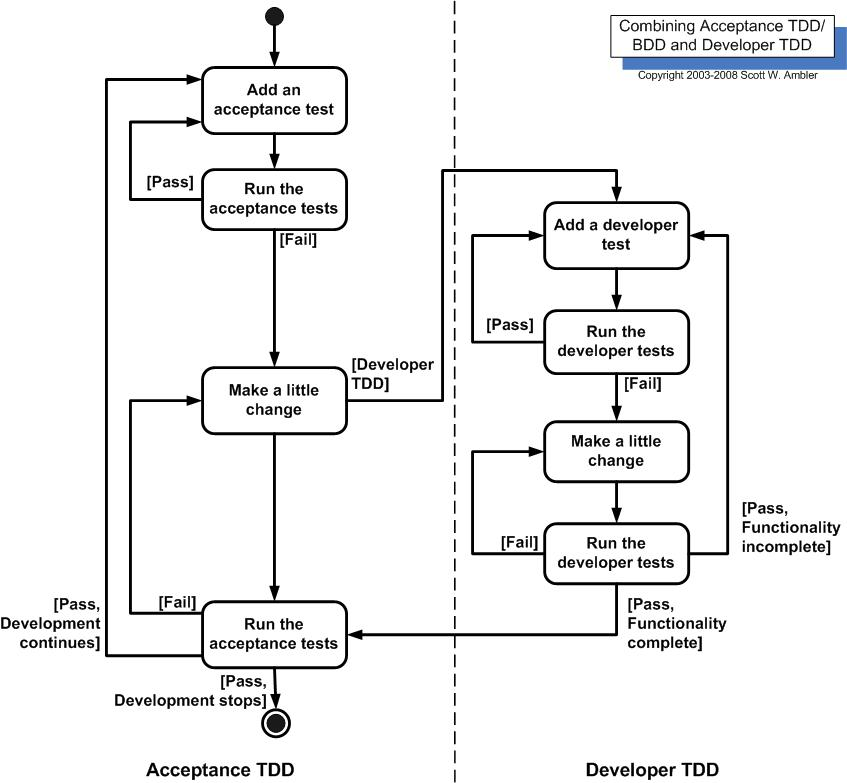
\includegraphics[width=\textwidth,height=0.8\textheight,keepaspectratio]{./images/atdd.jpg}
    \caption{Verschmelzung von Acceptance-Test-Driven Development und \enquote{Developer}-Test-Driven Development für Entwicklungsprozess \enquote{Scrum} \autocite{astels_2003}}
    \label{figure:atdd-dtdd}
\end{figure}

\section{Projektmanagersicht}
\subsection{Zeitmanagement}

Was bedeutet TDD fuer die Estimates?
Lohnt sich Tests schreiben ueberhaupt?
Bedeuten Tests nicht, dass mehr Aufwand gebracht werden muss, "nutzlosen" Code zu produzieren?
Das ist doch eine Reduktion des Throughputs.
Iterationen sind doch eh schon kurz genug.
Wann soll ueberhaupt getestet werden?
Meist Sprints so kurz definiert, dass Entwickler mit Stories fertig werden.
Wenn die Story fertig ist, sollte also Sprint beendet werden.

Stories sollten erst fertig sein, wenn sie vernuenftig getestet sind.
Stories sollten IN dem Sprint getestet werden, in der sie ins Sprint Backlog getan wurden.
Testing in agilen Entwicklungsprozessen sollte nicht designed werden nach dem Konzept, dass Testing auf den letzten Sprint arbeitet.
Immer momentanen Sprint testen, daher auch dafuer Zeit nehmen!

\chapter{Fazit}

Alles in einem ist es ersichtlich, dass TDD innerhalb von Scrum erhebliche Vorteile bietet, die viele Lücken füllt, die initial bestehen.
Man darf jedoch nicht vergessen, dass die Nutzung von TDD die Anforderungen an den einzelnen Entwickler immens steigert.
Nicht nur die Verantwortung jedes einzelnen steigt, aber auch die benötigte Disziplin.
Sollte TDD in Form von nicht-geschriebenen Tests vernachlässigt werden, so wirkt sich das auf die Wirksamkeit des gesamten Teams aus und hat eventuell schwerere Folgen, die ohne explizites Gegenwirken dazuführen, dass eine Menge an \enquote{Technical Debt} aufgebaut wird.
Diesem gegenüber stehenden ist die implizit als Wert vermittelte Eigenschaft \enquote{Whole-Team-Approach} des Scrum-Entwicklungsprozesses.
Das Team stellt sich dem Projekt gemeinsam, darf aber nicht vergessen, dass es autonom handelt und daher jeder hier auftretende Mangel folglich ihnen selbst, dem Produkt und somit ihrer Firma schadet.
Trotz dieses Problems überwiegen die Vorteile von TDD und, sollte es richtig implementiert und angewendet werden, zeigt auf, dass durch solch eine \enquote{simple} Methode Scrum zu einem Kinderspiel werden kann.

Leider konnte in Rahmen dieser kurzen Ausarbeitung kein Fokus auf andere, interessante Aspekte von agilen Testmethoden Rücksicht genommen werden.
Komplett ignoriert wurde beispielsweise die Analyse von TDD im Bezug auf die einzelnen Scrum-Rollen sowie auf die Komposition des Scrum-Teams.

\nocite{*}
\printbibliography

\begin{appendices}

  \KOMAoption{headsepline}{false}

\chapter{Überblick auf Test-Driven Development}
\begin{figure}[!htb]
  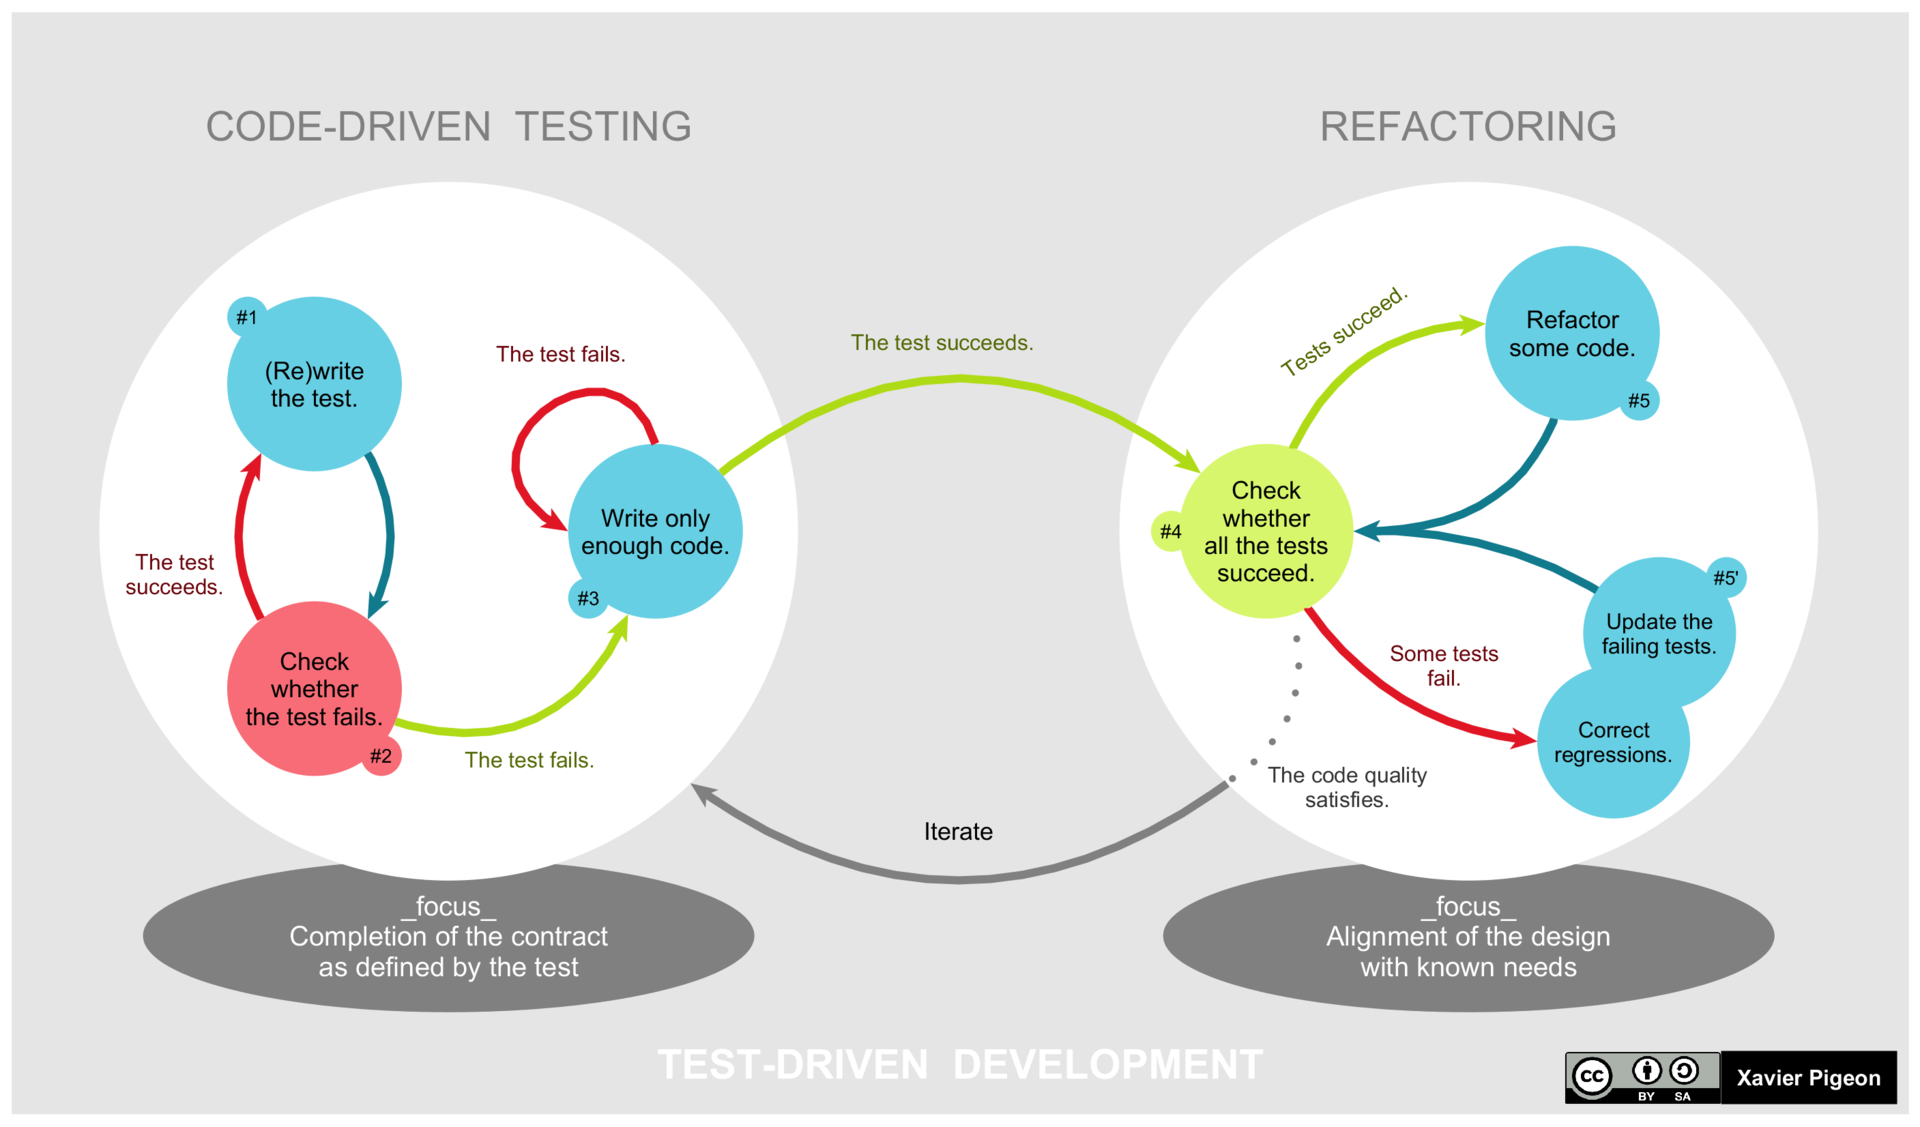
\includegraphics[width=\textwidth,height=0.85\textheight,keepaspectratio]{./images/1920px-TDD_Global_Lifecycle.png}
  \caption{Quelle: \autocite{TDD.Picture}}
  \label{figure:tdd-overview}
\end{figure}

\chapter{Überblick auf Entwicklungsprozess \enquote{Scrum}}
\begin{figure}[!htb]
  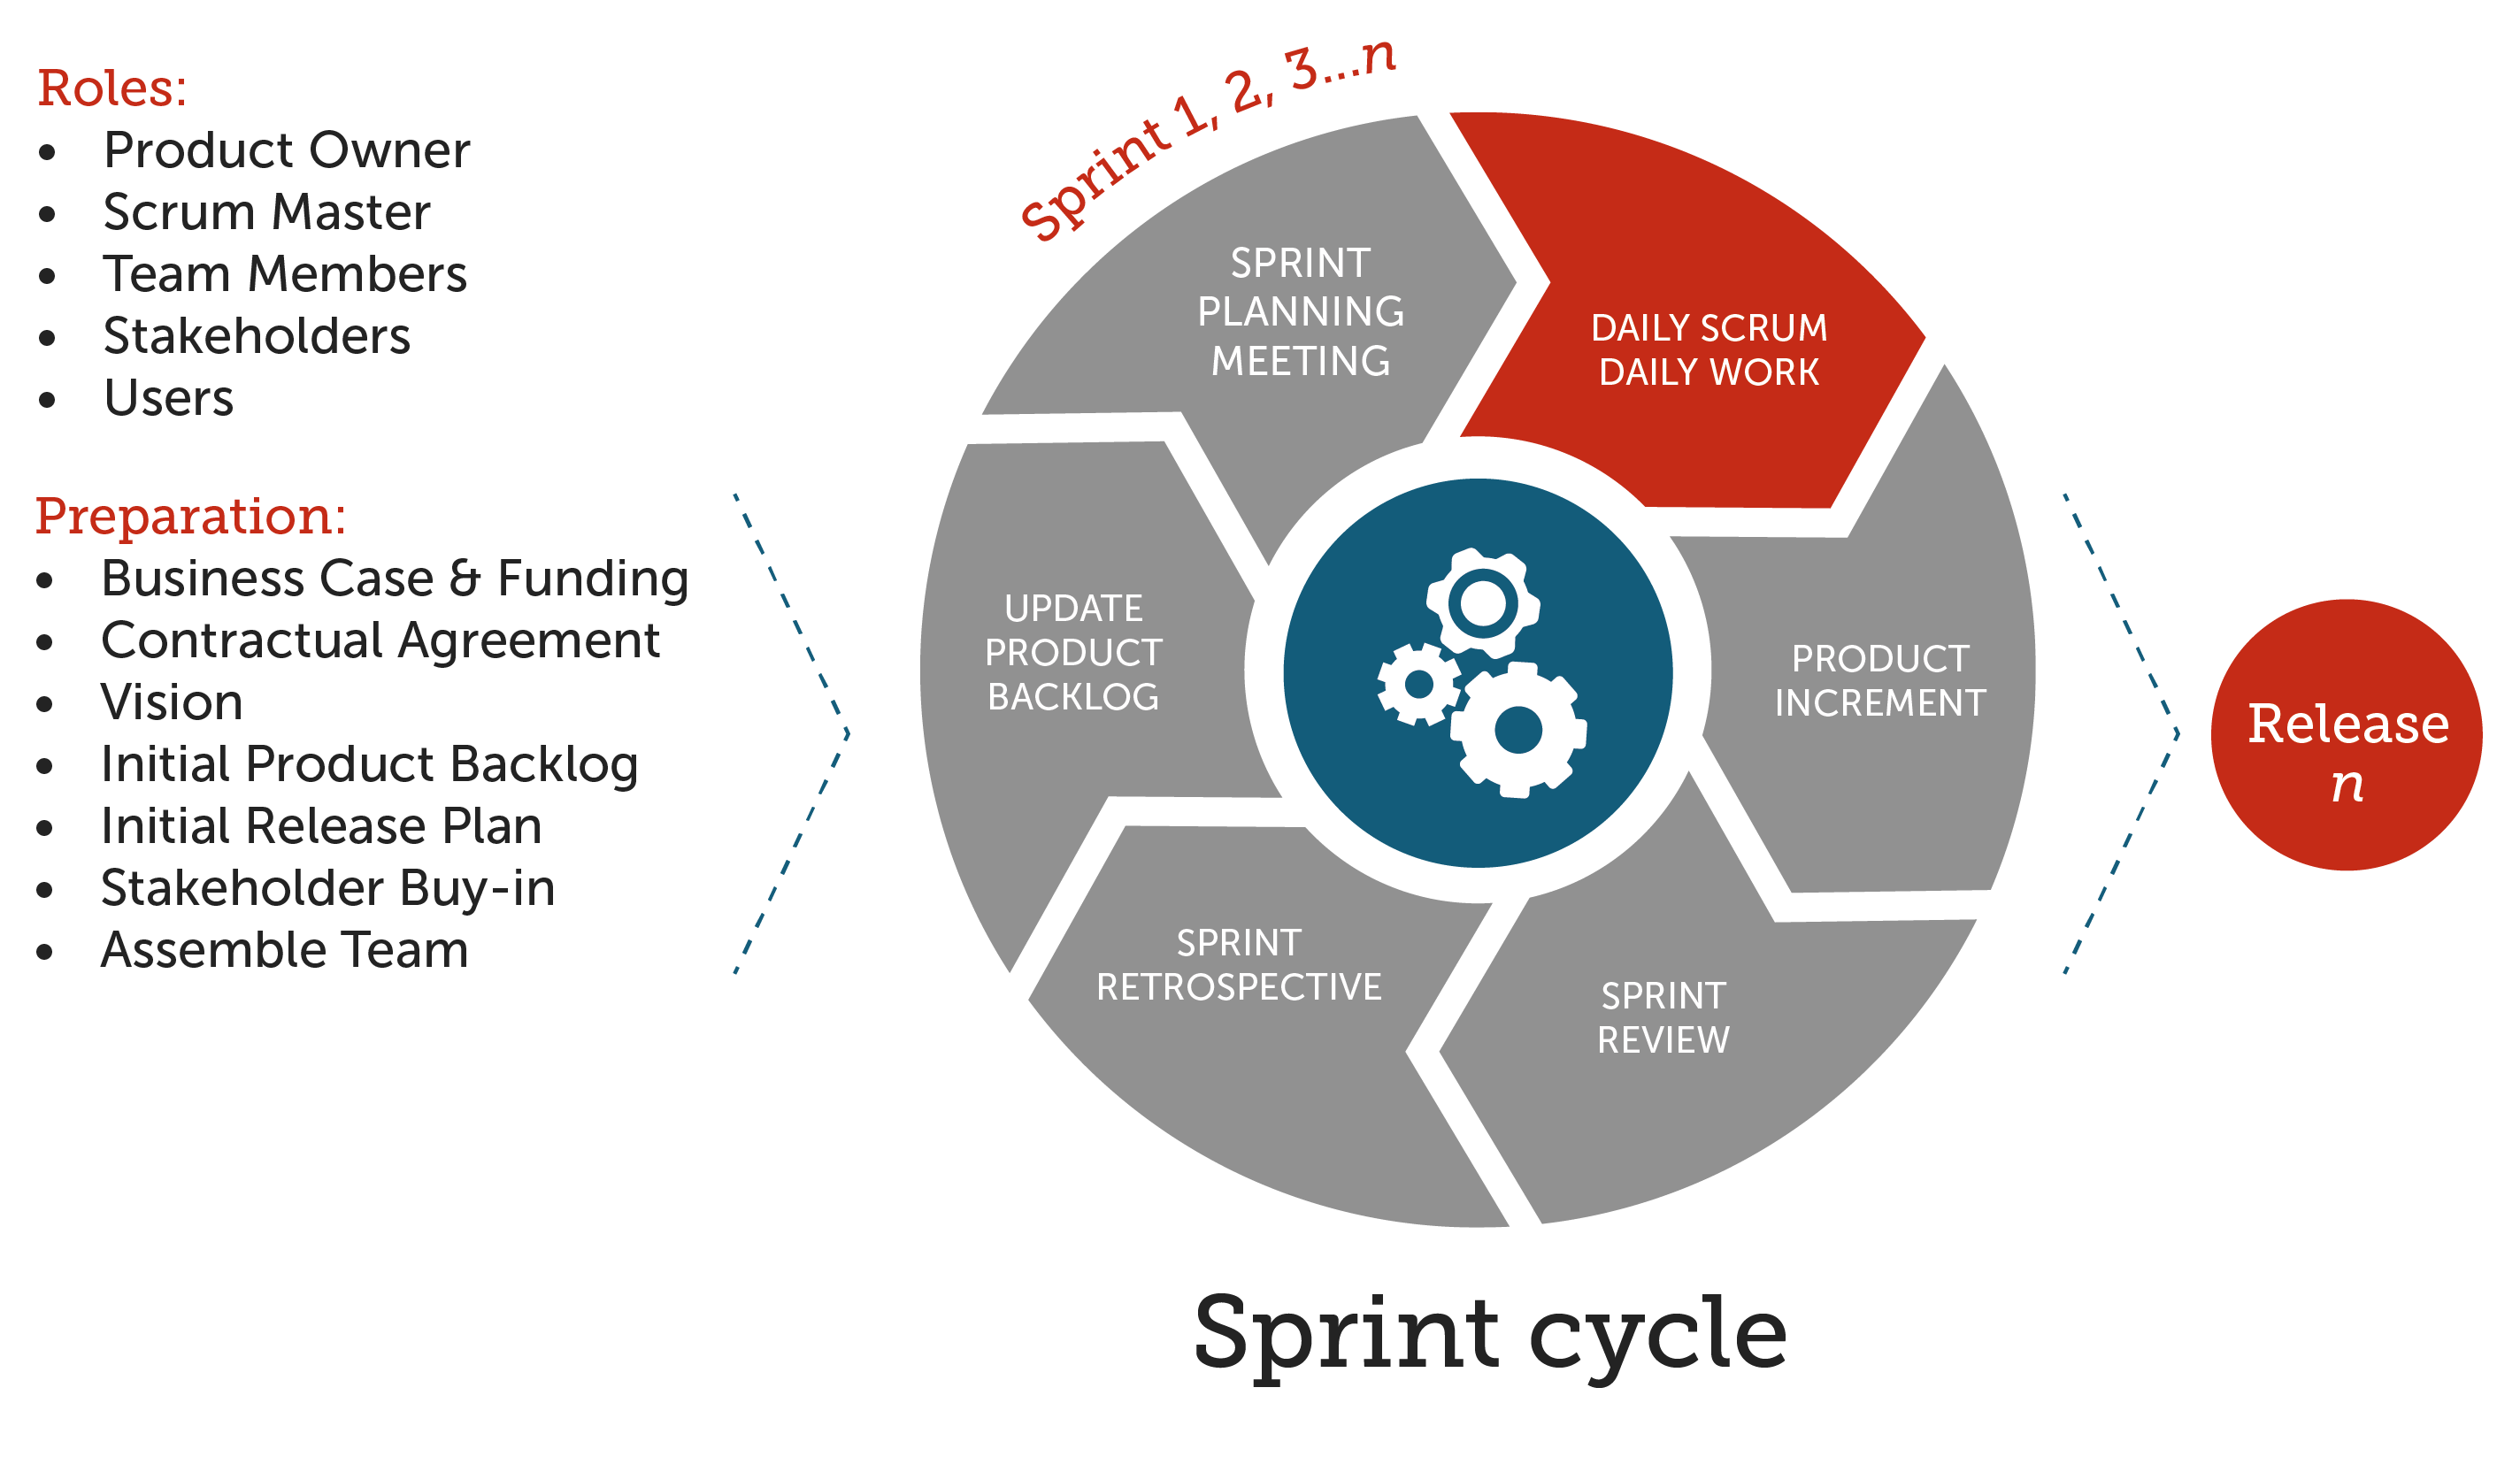
\includegraphics[width=\textwidth,height=0.9\textheight,keepaspectratio]{./images/the-daily-scrum-in-the-sprint-cycle.png}
  \caption{Quelle: \autocite{ManifestoDigital}}
  \label{figure:scrum-overview}
\end{figure}

\end{appendices}
% Can be used to add a list of acronyms with their description
%\glsaddall
%\deftranslation{to=German}{Acronyms}{Abkürzungsverzeichnis}
%\deftranslation{to=German}{Glossary}{Glossar}
%\printacronyms[title=Abkürzungsverzeichnis,toctitle=Abkürzungsverzeichnis]
%\printglossary[type=main]

%\addcontentsline{toc}{chapter}{\listfigurename}
%\listoffigures      % Abbildungsverzeichnis

%s\addcontentsline{toc}{chapter}{\listtablename}
% \listoftables       % Tabellenverzeichnis

\end{document}
